%        File: arfc-beamer.tex
%     Created: Sun May 5 10:00 PM 2013 C
%


%\documentclass[11pt,handout]{beamer}
\documentclass[9pt]{beamer}
\usetheme[white]{Illinois}
%\title[short title]{long title}
\title[Updating Fuel Cycle Assumptions]{Updates to time, power, and deployment in advanced reactor fuel cycle modeling}
%\subtitle[short subtitle]{long subtitle}
\subtitle[Short SubTitle]{ORNL Symposium}
%\author[short name]{long name}
\author[Nathan Ryan]{Nathan Ryan\\Advanced Reactors and Fuel Cycles}
%\date[short date]{long date}
\date[03.27.2025]{March 27, 2025}
%\institution[short name]{long name}
\institute[UIUC]{University of Illinois Urbana-Champaign}

%\usepackage{bbding}
\usepackage{amsfonts}
% \usepackage{algorithm}
% \usepackage[ruled]{algorithm2e}
% \usepackage{algorithmic}
\usepackage{algpseudocode}
% \usepackage{algorithmic}
% \usepackage{array}
\usepackage{amsmath}
\usepackage{xspace}
\usepackage{graphicx}
\usepackage{subfigure}
\usepackage{booktabs} % nice rules for tables
\usepackage{microtype} % if using PDF
\usepackage{bigints}
\usepackage{caption}
\usepackage{xcolor}
\usepackage{tikz}
\usetikzlibrary{shapes,arrows}


\definecolor{lightpurple}{HTML}{ECD9ED}
\definecolor{lightgreen}{HTML}{CAE0AB}

\tikzstyle{block} = [rectangle, draw, fill=lightgreen!20, text width=5em, text centered, rounded corners, node distance=4cm, minimum height=4em]
\tikzstyle{line} = [draw, -latex']

\newcommand{\cycamore}{\textsc{Cycamore}\xspace}
\newcommand{\cyclus}{\textsc{Cyclus}\xspace}

\newcommand{\units}[1] {\:\text{#1}}%
\newcommand{\SN}{S$_N$}%{S$_\text{N}$}%{$S_N$}%
\DeclareMathOperator{\erf}{erf}
%I need some complimentary error funcitons...
\DeclareMathOperator{\erfc}{erfc}
%Those icons in the references are terrible looking
\setbeamertemplate{bibliography item}[text]

%%%% Acronym support

\usepackage[acronym,toc]{glossaries}
%\newacronym{<++>}{<++>}{<++>}
\newacronym[longplural={metric tons of heavy metal}]{MTHM}{MTHM}{metric ton of heavy metal}
\newacronym{ABM}{ABM}{agent-based modeling}
\newacronym{ACDIS}{ACDIS}{Program in Arms Control \& Domestic and International Security}
\newacronym{AHTR}{AHTR}{Advanced High Temperature Reactor}
\newacronym{ANDRA}{ANDRA}{Agence Nationale pour la gestion des D\'echets RAdioactifs, the French National Agency for Radioactive Waste Management}
\newacronym{ANL}{ANL}{Argonne National Laboratory}
\newacronym{API}{API}{application programming interface}
\newacronym{ARE}{ARE}{Aircraft Reactor Experiment}
\newacronym{ARFC}{ARFC}{Advanced Reactors and Fuel Cycles}
\newacronym{ASME}{ASME}{American Society of Mechanical Engineers}
\newacronym{ATWS}{ATWS}{Anticipated Transient Without Scram}
\newacronym{BDBE}{BDBE}{Beyond Design Basis Event}
\newacronym{BIDS}{BIDS}{Berkeley Institute for Data Science}
\newacronym{CAFCA}{CAFCA}{ Code for Advanced Fuel Cycles Assessment }
\newacronym{CDTN}{CDTN}{Centro de Desenvolvimento da Tecnologia Nuclear}
\newacronym{CEA}{CEA}{Commissariat \`a l'\'Energie Atomique et aux \'Energies Alternatives}
\newacronym{CI}{CI}{continuous integration}
\newacronym{CNEN}{CNEN}{Comiss\~{a}o Nacional de Energia Nuclear}
\newacronym{CNERG}{CNERG}{Computational Nuclear Engineering Research Group}
\newacronym{COSI}{COSI}{Commelini-Sicard}
\newacronym{COTS}{COTS}{commercial, off-the-shelf}
\newacronym{CSNF}{CSNF}{commercial spent nuclear fuel}
\newacronym{CTAH}{CTAHs}{Coiled Tube Air Heaters}
\newacronym{CUBIT}{CUBIT}{CUBIT Geometry and Mesh Generation Toolkit}
\newacronym{CURIE}{CURIE}{Centralized Used Fuel Resource for Information Exchange}
\newacronym{DAG}{DAG}{directed acyclic graph}
\newacronym{DANESS}{DANESS}{Dynamic Analysis of Nuclear Energy System Strategies}
\newacronym{DBE}{DBE}{Design Basis Event}
\newacronym{DESAE}{DESAE}{Dynamic Analysis of Nuclear Energy Systems Strategies}
\newacronym{DHS}{DHS}{Department of Homeland Security}
\newacronym{DOE}{DOE}{Department of Energy}
\newacronym{DRACS}{DRACS}{Direct Reactor Auxiliary Cooling System}
\newacronym{DRE}{DRE}{dynamic resource exchange}
\newacronym{DSNF}{DSNF}{DOE spent nuclear fuel}
\newacronym{DYMOND}{DYMOND}{Dynamic Model of Nuclear Development }
\newacronym{EBS}{EBS}{Engineered Barrier System}
\newacronym{EDZ}{EDZ}{Excavation Disturbed Zone}
\newacronym{EIA}{EIA}{U.S. Energy Information Administration}
\newacronym{EPA}{EPA}{Environmental Protection Agency}
\newacronym{EP}{EP}{Engineering Physics}
\newacronym{FCO}{FCO}{Fuel Cycle Options}
\newacronym{FCT}{FCT}{Fuel Cycle Technology}
\newacronym{FEHM}{FEHM}{Finite Element Heat and Mass Transfer}
\newacronym{FEPs}{FEPs}{Features, Events, and Processes}
\newacronym{FHR}{FHR}{Fluoride-Salt-Cooled High-Temperature Reactor}
\newacronym{FLiBe}{FLiBe}{Fluoride-Lithium-Beryllium}
\newacronym{GDSE}{GDSE}{Generic Disposal System Environment}
\newacronym{GDSM}{GDSM}{Generic Disposal System Model}
\newacronym{GENIUSv1}{GENIUSv1}{Global Evaluation of Nuclear Infrastructure Utilization Scenarios, Version 1}
\newacronym{GENIUSv2}{GENIUSv2}{Global Evaluation of Nuclear Infrastructure Utilization Scenarios, Version 2}
\newacronym{GENIUS}{GENIUS}{Global Evaluation of Nuclear Infrastructure Utilization Scenarios}
\newacronym{GPAM}{GPAM}{Generic Performance Assessment Model}
\newacronym{GRSAC}{GRSAC}{Graphite Reactor Severe Accident Code}
\newacronym{GUI}{GUI}{graphical user interface}
\newacronym{HLW}{HLW}{high level waste}
\newacronym{HPC}{HPC}{high-performance computing}
\newacronym{HTC}{HTC}{high-throughput computing}
\newacronym{HTGR}{HTGR}{High Temperature Gas-Cooled Reactor}
\newacronym{IAEA}{IAEA}{International Atomic Energy Agency}
\newacronym{IEMA}{IEMA}{Illinois Emergency Mangament Agency}
\newacronym{INL}{INL}{Idaho National Laboratory}
\newacronym{IPRR1}{IRP-R1}{Instituto de Pesquisas Radioativas Reator 1}
\newacronym{IRP}{IRP}{Integrated Research Project}
\newacronym{ISFSI}{ISFSI}{Independent Spent Fuel Storage Installation}
\newacronym{ISRG}{ISRG}{Independent Student Research Group}
\newacronym{JFNK}{JFNK}{Jacobian-Free Newton Krylov}
\newacronym{LANL}{LANL}{Los Alamos National Laboratory}
\newacronym{LBNL}{LBNL}{Lawrence Berkeley National Laboratory}
\newacronym{LCOE}{LCOE}{levelized cost of electricity}
\newacronym{LDRD}{LDRD}{laboratory directed research and development}
\newacronym{LFR}{LFR}{Lead-Cooled Fast Reactor}
\newacronym{LLNL}{LLNL}{Lawrence Livermore National Laboratory}
\newacronym{LMFBR}{LMFBR}{Liquid Metal Fast Breeder Reactor}
\newacronym{LOFC}{LOFC}{Loss of Forced Cooling}
\newacronym{LOHS}{LOHS}{Loss of Heat Sink}
\newacronym{LOLA}{LOLA}{Loss of Large Area}
\newacronym{LP}{LP}{linear program}
\newacronym{MA}{MA}{minor actinide}
\newacronym{MCNP}{MCNP}{Monte Carlo N-Particle code}
\newacronym{MILP}{MILP}{mixed-integer linear program}
\newacronym{MIT}{MIT}{the Massachusetts Institute of Technology}
\newacronym{MOAB}{MOAB}{Mesh-Oriented datABase}
\newacronym{MOOSE}{MOOSE}{Multiphysics Object-Oriented Simulation Environment}
\newacronym{MOX}{MOX}{mixed oxide}
\newacronym{MSBR}{MSBR}{Molten Salt Breeder Reactor}
\newacronym{MSRE}{MSRE}{Molten Salt Reactor Experiment}
\newacronym{MSR}{MSR}{Molten Salt Reactor}
\newacronym{NAGRA}{NAGRA}{National Cooperative for the Disposal of Radioactive Waste}
\newacronym{NEAMS}{NEAMS}{Nuclear Engineering Advanced Modeling and Simulation}
\newacronym{NEUP}{NEUP}{Nuclear Energy University Programs}
\newacronym{NFCSim}{NFCSim}{Nuclear Fuel Cycle Simulator}
\newacronym{NGNP}{NGNP}{Next Generation Nuclear Plant}
\newacronym{NMWPC}{NMWPC}{Nuclear MW Per Capita}
\newacronym{NNSA}{NNSA}{National Nuclear Security Administration}
\newacronym{NPRE}{NPRE}{Department of Nuclear, Plasma, and Radiological Engineering}
\newacronym{NQA1}{NQA-1}{Nuclear Quality Assurance - 1}
\newacronym{NRC}{NRC}{Nuclear Regulatory Commission}
\newacronym{NSF}{NSF}{National Science Foundation}
\newacronym{NSSC}{NSSC}{Nuclear Science and Security Consortium}
\newacronym{NUWASTE}{NUWASTE}{Nuclear Waste Assessment System for Technical Evaluation}
\newacronym{NWF}{NWF}{Nuclear Waste Fund}
\newacronym{NWTRB}{NWTRB}{Nuclear Waste Technical Review Board}
\newacronym{OCRWM}{OCRWM}{Office of Civilian Radioactive Waste Management}
\newacronym{ORION}{ORION}{ORION}
\newacronym{ORNL}{ORNL}{Oak Ridge National Laboratory}
\newacronym{PARCS}{PARCS}{Purdue Advanced Reactor Core Simulator}
\newacronym{PBAHTR}{PB-AHTR}{Pebble Bed Advanced High Temperature Reactor}
\newacronym{PBFHR}{PB-FHR}{Pebble-Bed Fluoride-Salt-Cooled High-Temperature Reactor}
\newacronym{PEI}{PEI}{Peak Environmental Impact}
\newacronym{PH}{PRONGHORN}{PRONGHORN}
\newacronym{PRKE}{PRKE}{Point Reactor Kinetics Equations}
\newacronym{PSPG}{PSPG}{Pressure-Stabilizing/Petrov-Galerkin}
\newacronym{PWAR}{PWAR}{Pratt and Whitney Aircraft Reactor}
\newacronym{PWR}{PWR}{Pressurized Water Reactor}
\newacronym{PyNE}{PyNE}{Python toolkit for Nuclear Engineering}
\newacronym{PyRK}{PyRK}{Python for Reactor Kinetics}
\newacronym{QA}{QA}{quality assurance}
\newacronym{RDD}{RD\&D}{Research Development and Demonstration}
\newacronym{RD}{R\&D}{Research and Development}
\newacronym{RELAP}{RELAP}{Reactor Excursion and Leak Analysis Program}
\newacronym{RIA}{RIA}{Reactivity Insertion Accident}
\newacronym{RIF}{RIF}{Region-Institution-Facility}
\newacronym{SFR}{SFR}{Sodium-Cooled Fast Reactor}
\newacronym{SINDAG}{SINDA{\textbackslash}G}{Systems Improved Numerical Differencing Analyzer $\backslash$ Gaski}
\newacronym{SKB}{SKB}{Svensk K\"{a}rnbr\"{a}nslehantering AB}
\newacronym{SNF}{SNF}{spent nuclear fuel}
\newacronym{SNL}{SNL}{Sandia National Laboratory}
\newacronym{STC}{STC}{specific temperature change}
\newacronym{SUPG}{SUPG}{Streamline-Upwind/Petrov-Galerkin}
\newacronym{SWF}{SWF}{Separations and Waste Forms}
\newacronym{SWU}{SWU}{Separative Work Unit}
\newacronym{TRIGA}{TRIGA}{Training Research Isotope General Atomic}
\newacronym{TRISO}{TRISO}{Tristructural Isotropic}
\newacronym{TSM}{TSM}{Total System Model}
\newacronym{TSPA}{TSPA}{Total System Performance Assessment for the Yucca Mountain License Application}
\newacronym{ThOX}{ThOX}{thorium oxide}
\newacronym{UFD}{UFD}{Used Fuel Disposition}
\newacronym{UML}{UML}{Unified Modeling Language}
\newacronym{UOX}{UOX}{uranium oxide}
\newacronym{UQ}{UQ}{uncertainty quantification}
\newacronym{US}{US}{United States}
\newacronym{UW}{UW}{University of Wisconsin}
\newacronym{VISION}{VISION}{the Verifiable Fuel Cycle Simulation Model}
\newacronym{VV}{V\&V}{verification and validation}
\newacronym{WIPP}{WIPP}{Waste Isolation Pilot Plant}
\newacronym{YMR}{YMR}{Yucca Mountain Repository Site}
\newacronym{leup}{LEU+}{LEU Plus}

\newacronym{ever}{EVER}{Enrichment Versatile non-Equilibrium Reactor}
\newacronym{clover}{CLOVER}{Core LOading Versatile non-Equilibrium Reactor}
\newacronym{dpr}{DPR}{Dynamic Power Reactor}
\newacronym{tod}{TOD}{Trading On-Demand}

\makeglossaries

%try to get rid of header on title page\dots
\makeatletter
    \newenvironment{withoutheadline}{
        \setbeamertemplate{headline}[default]
        \def\beamer@entrycode{\vspace*{-\headheight}}
    }{}
\makeatother

% \makeatother
% \setbeamertemplate{footline}
% {
%   \leavevmode%
%   \hbox{%
%     \rightline{\insertframenumber{} / \inserttotalframenumber\hspace*{1ex}}
%   }%
%   \vskip0pt%
% }
% \makeatletter
\setbeamertemplate{caption}{\raggedright\insertcaption\par}
\setbeamertemplate{page number in head/foot}[appendixframenumber]
\setbeamertemplate{caption}[numbered]

\begin{document}
%%%%%%%%%%%%%%%%%%%%%%%%%%%%%%%%%%%%%%%%%%%%%%%%%%%%%%%%%%%%%
%% From uw-beamer Here's a handy bit of code to place at
%% the beginning of your presentation (after \begin{document}):
\newcommand*{\alphabet}{ABCDEFGHIJKLMNOPQRSTUVWXYZabcdefghijklmnopqrstuvwxyz}
\newlength{\highlightheight}
\newlength{\highlightdepth}
\newlength{\highlightmargin}
\setlength{\highlightmargin}{2pt}
\settoheight{\highlightheight}{\alphabet}
\settodepth{\highlightdepth}{\alphabet}
\addtolength{\highlightheight}{\highlightmargin}
\addtolength{\highlightdepth}{\highlightmargin}
\addtolength{\highlightheight}{\highlightdepth}
\newcommand*{\Highlight}{\rlap{\textcolor{HighlightBackground}{\rule[-\highlightdepth]{\linewidth}{\highlightheight}}}}
%%%%%%%%%%%%%%%%%%%%%%%%%%%%%%%%%%%%%%%%%%%%%%%%%%%%%%%%%%%%%
%%--------------------------------%%
\begin{withoutheadline}
\frame{
  \titlepage
}
\end{withoutheadline}

%%--------------------------------%%
\AtBeginSection[]{
\begin{frame}
  \frametitle{Outline}
  \tableofcontents[currentsection]
\end{frame}
}
\section{Background}
\subsection{My Background}

  \begin{frame}
    \frametitle{Know how to code?}
    Consider volunteering in lessons or mentoring in the Computational Resource Access NEtwork (CRANE) so we can support more students!
    \begin{figure}
        \centering
        
\includegraphics[width=0.65\textwidth]{images/CRANE_logo_inverted.png}
    \end{figure}
    Go to our website: \url{https://www.cranephysics.org}
  \end{frame}

  \begin{frame}
    \frametitle{Removing assumptions in nuclear fuel cycle modeling.}
    % The through line of my research is using computational tools to remove
    % assumptions.
    % \vspace{0.6cm}
    \begin{columns}
      \column[t]{5cm}
      I am a Masters student in the Advanced Reactors and Fuel Cycles group at
      UIUC under Prof. Madicken Munk and Prof. Kathryn Huff.
      \begin{center}
              
\includegraphics[height=0.2\textheight]{./images/arfc-logo}
      \end{center}

      \column[t]{5cm}
      I earned my B.S. in Engineering Physics from UIUC.
      \begin{figure}[htbp!]
        \begin{center}
          
\includegraphics[height=3cm]{./images/ill_phys.png}
        \end{center}
        % \caption{A caption describing the image. \cite{lastname_firstword_1900}.}
        \label{fig:uiuc_phys}
      \end{figure}
    \end{columns}\pause
    \begin{itemize}[<+->]
      \item Making transaction models more detailed.
      \item Identifying realtime diversion or diversion paths.
      \item Making facility models more accurate.
      \item Finding advanced reactor impacts on the fuel cycle.
    \end{itemize}
  \end{frame}


\section{Nuclear Fuel Cycle}
\subsection{Fuel Cycle Overview}

  \begin{frame}
      \frametitle{Generally, fuel cycles have these steps.}
      \begin{figure}[ht!]
      \centering
      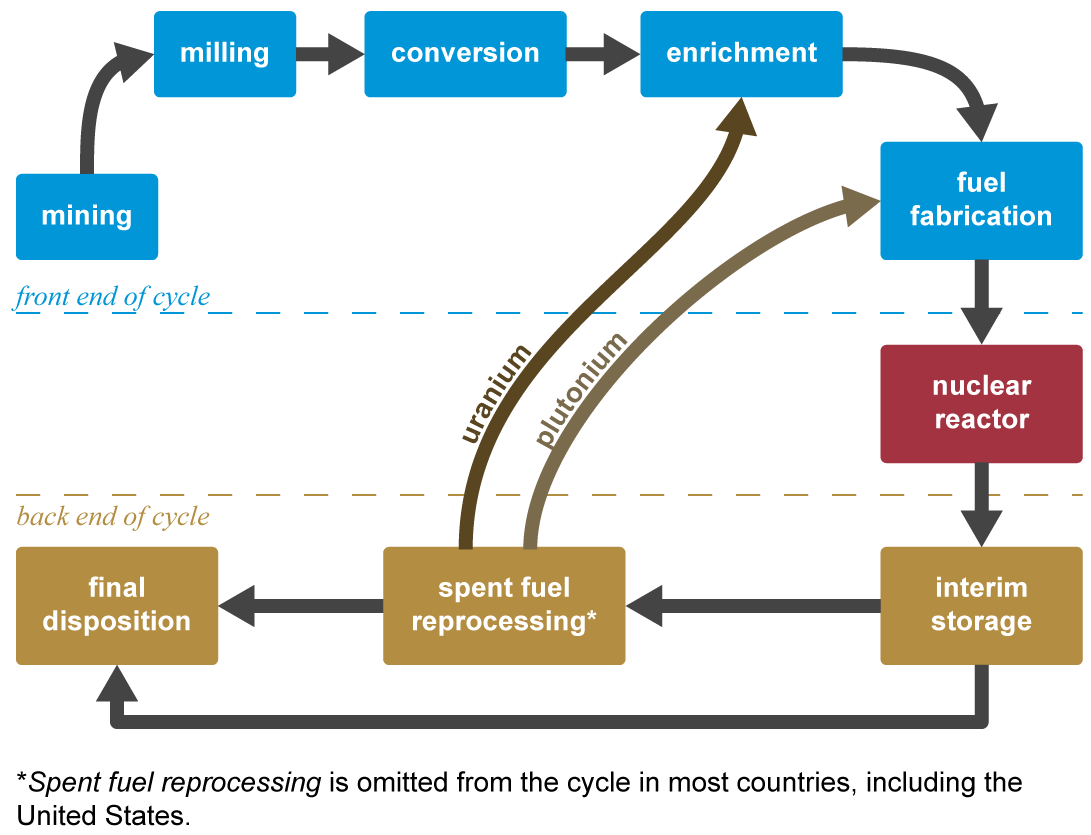
\includegraphics[width=0.65\textwidth]{images/nuclear_fuel_cycle.png}
      \caption{General nuclear fuel cycle overview \cite{penn_fc}.}
      \end{figure}
  \end{frame}

  \begin{frame}
      \frametitle{Not all fuel cycles are made equal, and we want options.}
      Analysis of the economics, waste generation, proliferation risk, and sustainability motivate the need for options. With metrics like:
        \begin{itemize}%[<+->]
            \item natural resource utilization, % mention or-sage
            \item waste mass/volume,
            \item special material quantities,
            \item separative work units,
            \item and energy production,
        \end{itemize}
        we can evaluate the tradeoffs between fuel cycle options.
  \end{frame}

  \begin{frame}
    \frametitle{We use \cyclus to model fuel cycles.}
    \vspace{10pt}
    \cyclus is an open-source agent-based fuel cycle code allowing for detailed facility and transaction modeling \cite{huff_fundamental_2016}.
    % \vspace{10pt}
    \begin{center}
    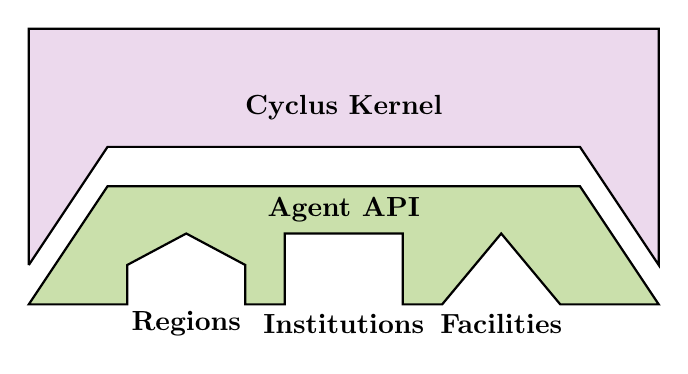
\begin{tikzpicture}
      % Main rectangle
      \draw[thick, fill=lightpurple] (0,0) -- (1,1.5) -- (7, 1.5) -- (8,0) -- (8,3) -- (0,3) -- (0,0);
      \node at (4,2) {\textbf{Cyclus Kernel}};

      % Trapezoid cut-out at the bottom
      \draw[thick, fill=lightgreen] (0,-0.5) -- (1,1) -- (7,1) -- (8,-0.5) -- (6.75, -0.5) -- (6, 0.4) -- (5.25, -0.5) -- (4.75, -0.5) -- (4.75, 0.4) -- (3.25, 0.4) -- (3.25, -0.5) -- (2.75, -0.5) -- (2.75, 0.0) -- (2, 0.4) -- (1.25, 0.0) -- (1.25, -0.5) -- cycle;
      \node at (4,0.7) {\textbf{Agent API}};
      \node at (2, -0.75) {\textbf{Regions}};
      % \node at (2, -1.1) {\textbf{API}};

      \node at (4, -0.75) {\textbf{Institutions}};
      % \node at (4, -1.1) {\textbf{API}};

      \node at (6, -0.75) {\textbf{Facilities}};
      % \node at (6, -1.1) {\textbf{API}};
    \end{tikzpicture}
  \end{center} \pause

  The \cyclus ecosystem has many \textit{archetypes}, or generic facility models, (like the \cycamore Reactor) that can be used to model different fuel cycle facilities.
  \end{frame}

  \begin{frame}
    \frametitle{\cyclus is being used to tackle big questions.}
    \begin{block}{Transaction Models.}
        There is active work to incorporate realistic purchasing agreements and market models into \cyclus.
    \end{block} \pause
    \begin{block}{Nonproliferation and Safeguards.}
        CNTAUR \cite{mummah_advanced_2024} and Pyre \cite{westphal_modeling_2019} format outputs in IAEA code 10 format and model real time diversion, respectively.
    \end{block} \pause
    \begin{block}{Facility Models.}
      OpenMCyclus \cite{openmcyclus_paper} couples \cyclus with OpenMC to model realtime depletion. From my work, we will discuss the \gls{dpr}, \gls{tod} reactor, and \gls{ever} today.
  \end{block} \pause
    \begin{block}{Transition Scenarios.}
        We will talk about this in the context of advanced reactors.
    \end{block}
  \end{frame}

\section{Enrichment and Core Loading Versatility}
\subsection{2023 \cyclus NEUP}

\begin{frame}
  \frametitle{Illuminating Emerging Supply Chain and Waste Management
  Challenges.}
  My enrichment versatility work is one part of a broader effort to enhance the \cyclus fuel cycle code. The three areas of work are to:
  \begin{itemize}[<+->]
    \item improve modeling of supply chain dynamics,
    \item account for regional and temporal variability in material needs,
    \item and expand models appropriate for variations in reactor fueling strategies.
  \end{itemize}
\end{frame}

\begin{frame}
  \frametitle{Varying core loading improves fuel utilization.}
  Fuel cycle simulators often \cite{out_of_core} assume that:
  \begin{itemize}
    \item the utilization of each fuel assembly is the same,\pause
    \item and reactor power is constant over its lifetime when not refueling.\pause
  \end{itemize}
  In our models, these assumptions for the reactor and fuel are not necessarily connected.
\end{frame}

\begin{frame}
  \frametitle{EVER changes the primary fuel for a reactor.}
  The \cycamore reactor can prefer fuels, but a user could not require the reactor take in or output a specific fuel.
  \begin{figure}
  \centering
    \tikzstyle{line} = [draw, -latex']
    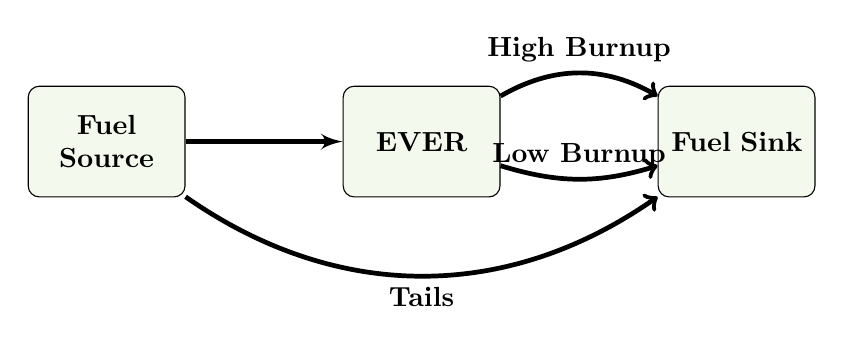
\begin{tikzpicture}[node distance = 5cm, auto]
        % Place nodes
        \node [block] (init) {\textbf{EVER}};
        \node [block, left of=init] (source) {\textbf{Fuel Source}};
        \node [block, right of=init] (sink) {\textbf{Fuel Sink}};

        % Draw edges
        \path [line, line width=0.6mm] (source) -- (init);

        \draw[->, line width=0.6mm] (init) edge[bend left] node[midway]{\textbf{High Burnup}} (sink);

        \draw[->, line width=0.6mm] (init) edge[bend right=17] node[above]{\textbf{Low Burnup}} (sink);

        \draw[->, line width=0.6mm] (source) edge[bend right=35] node[below]{\textbf{Tails}} (sink);
    \end{tikzpicture}
  \caption{The idea of the Enrichment Versatile non-Equilibrium Reactor (EVER).}
  \end{figure}
\end{frame}

% \begin{frame}
%   \frametitle{This toy scenario moves from HALEU to LEU.}
%   \begin{figure}
%     \centering
%     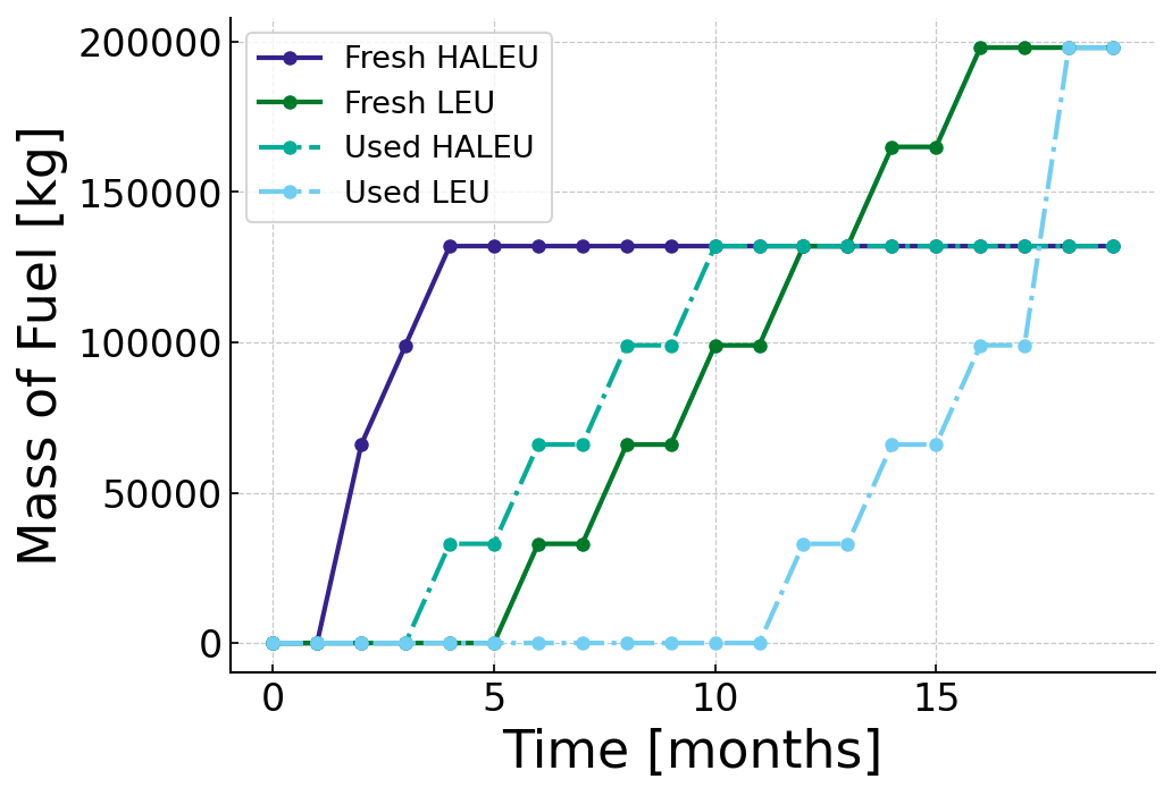
\includegraphics[width=0.65\textwidth]{images/mass_fuel.png}
%     \caption{The amount of fuel supplied to the reactor.}
%   \end{figure}
% \end{frame}

\begin{frame}
  \frametitle{The less-burnt fuel is visible in the stored isotopic contents.}
  \begin{figure}
    \centering
    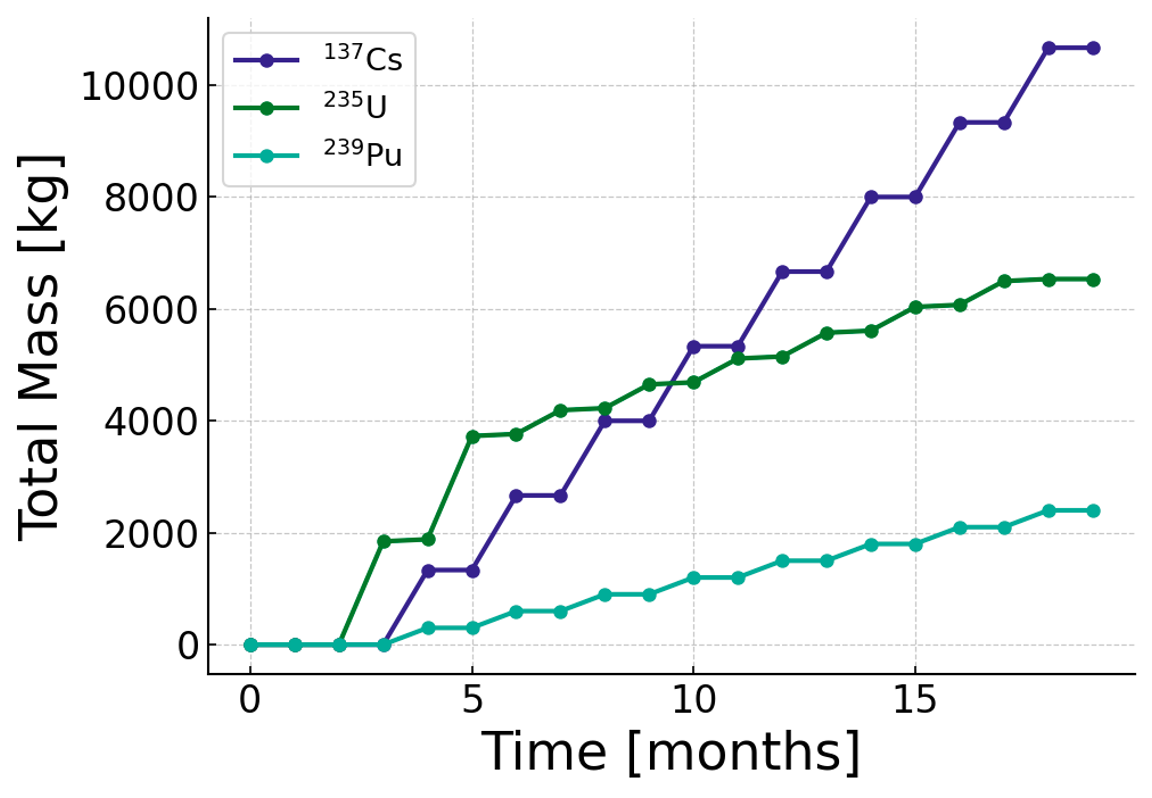
\includegraphics[width=0.65\textwidth]{images/mass_isotopes.png}
    \caption{The cumulative isotopes stored in the repository.}
  \end{figure}
\end{frame}

\subsection{Future Work}
\begin{frame}
  \frametitle{Future work on EVER.}
  \begin{itemize}[<+->]
    \item Pre-generate core-averaged cross sections and update group constant data.
    \item Vary recycling technology (PUREX, Electrolysis, Pyroprocessing).
    \item Incorporate different cooling, production, and processing times according to fuel type.
    \item Introduce the ability for the user to specify the location of fuel elements in the reactor core.
  \end{itemize}
\end{frame}

\section{Dynamic Power and On-Demand Trading}

\subsection{Dynamic Power Reactor}
\begin{frame}
  \frametitle{\cycamore's reactor assumes constant power.}
  Constant power means that energy-demand driven deployment will under-deploy reactors.
  \begin{figure}
    \centering
    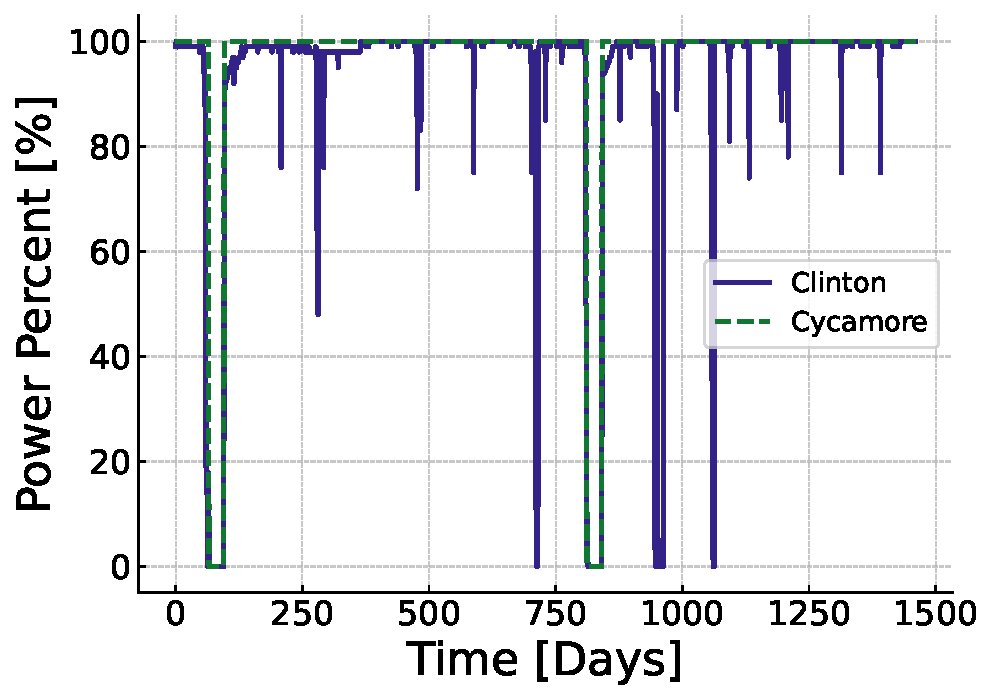
\includegraphics[width=0.65\textwidth]{images/power_percent_clinton_fake.pdf}
    \caption{Modeling Clinton's power with the \cycamore reactor over-predicted 62.2\% of the time.}
  \end{figure}
\end{frame}

% \begin{frame}
%   \frametitle{Using NRC data, we can modify the reactor's power capacity.}
%   \begin{figure}
%     \centering
%     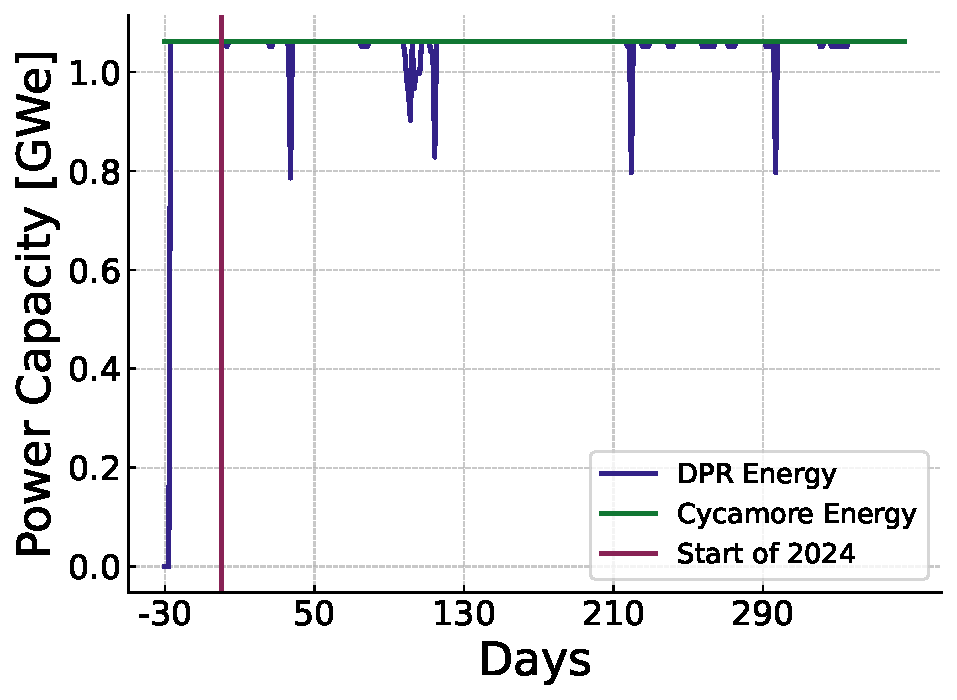
\includegraphics[width=0.65\textwidth]{images/dpr_cycamore_energy.pdf}
%     \caption{Comparing the DPR Clinton to the \cycamore Clinton.}
%   \end{figure}
% \end{frame}

\begin{frame}
  \frametitle{Clinton and the Dynamic Power Reactor's "Clinton" agree.}
  \begin{figure}
    \centering
    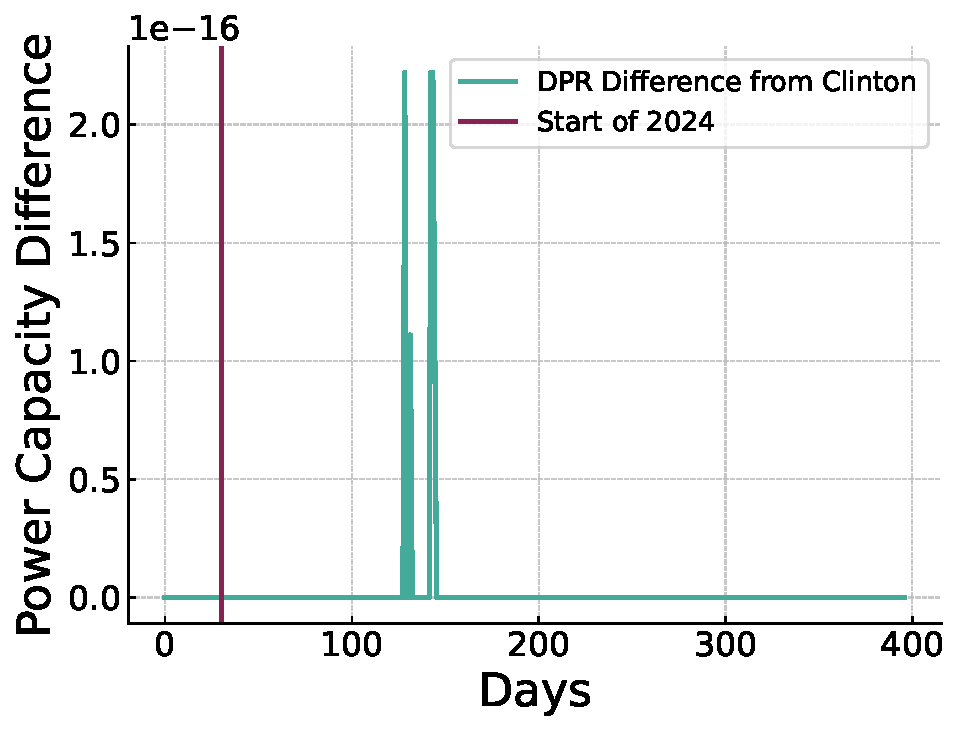
\includegraphics[width=0.65\textwidth]{images/dpr_diff.pdf}
    \caption{Max difference between Clinton and DPR is $2.22 \times 10^{-16}$.}
  \end{figure}
\end{frame}


\subsection{Trading On-Demand Reactor}
\begin{frame}
  \frametitle{A \cyclus time step has 3 parts.}
  After being built, every time step in a \cyclus simulation has 3 phases that the agents structure their behavior around before decommissioning:
  \begin{itemize}
    \item agents respond to current simulation state (Tick Phase), \pause
    \item resource exchange execution (Exchange Phase), \pause
    \item and agents reconcile their state (Tock Phase). \pause
  \end{itemize}
  \vspace{5pt}
  For example, when the \cycamore reactor refuels, it will: \pause
  \begin{itemize}[<+->]
    \item identify which fuel is ready to be discharged (Tick Phase),
    \item submit a bid for new fuel (Exchange Phase),
    \item then load new fuel (Tock Phase).
  \end{itemize}
\end{frame}

% \begin{frame}
%   \frametitle{\cyclus has a universal time step for all agents.}

% \end{frame}

% \begin{frame}
%   \frametitle{Using \gls{tod} resulted in a speedup of 1.038.}
%   \begin{figure}
%     \centering
%     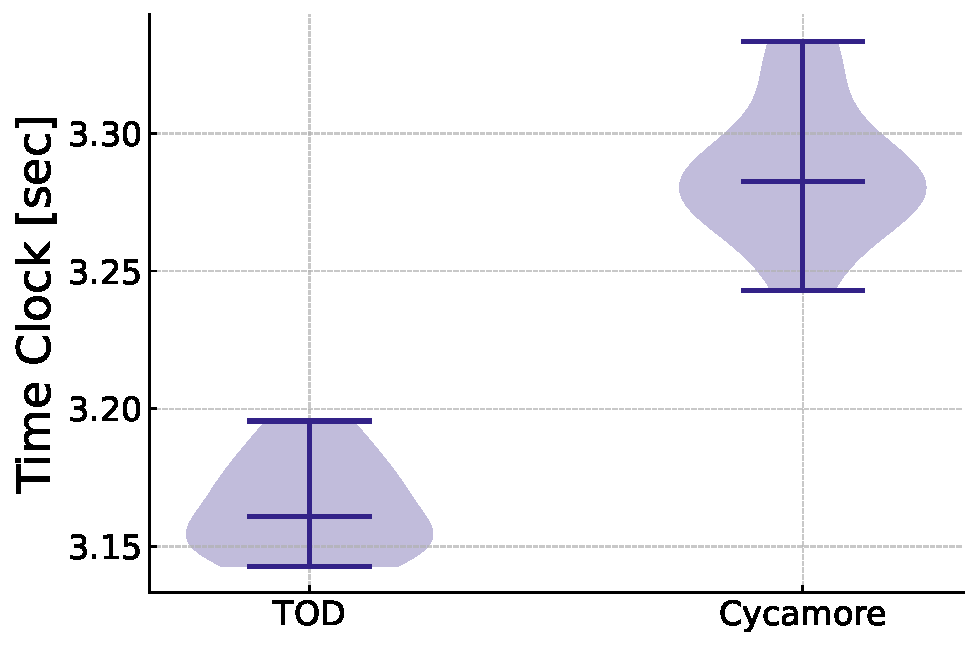
\includegraphics[width=0.65\textwidth]{images/time_clock_violin.pdf}
%     \caption{A-B-C simulation of the \cycamore reactor and the \gls{tod} reactor.}
%   \end{figure}
% \end{frame}

\begin{frame}
  \frametitle{The \gls{tod} reactor only submits a bid for fuel when it needs to.}
  Instead of checking the fuel at every time step, \gls{tod} calculates the next time it will need fuel and waits until then to trade. \pause

  \vspace{20pt}
  To compare the \cycamore reactor and \gls{tod} reactor, we create an A-B-C scenario for a fleet of each.
  \begin{center}
    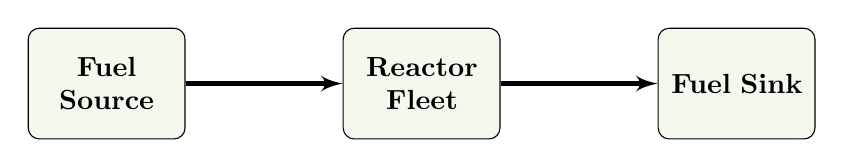
\begin{tikzpicture}[node distance = 2cm, auto]
        % Place nodes
        \node [block] (init) {\textbf{Reactor Fleet}};
        \node [block, left of=init] (expert) {\textbf{Fuel Source}};
        \node [block, right of=init] (sink) {\textbf{Fuel Sink}};
        % Draw edges
        \path [line, line width=0.6mm] (expert) -- (init);
        \path [line, line width=0.6mm] (init) -- (sink);
    \end{tikzpicture}
  \end{center}
\end{frame}

\begin{frame}
  \frametitle{The \gls{tod} reactor has a higher utilization than \cycamore.}
Across machines, we are interested in reducing the number of unnecessary trades, which corresponds to reducing the number of instructions executed by the reactor. \pause
  \begin{columns}
    \column[t]{5cm}
    \begin{figure}
      \centering
      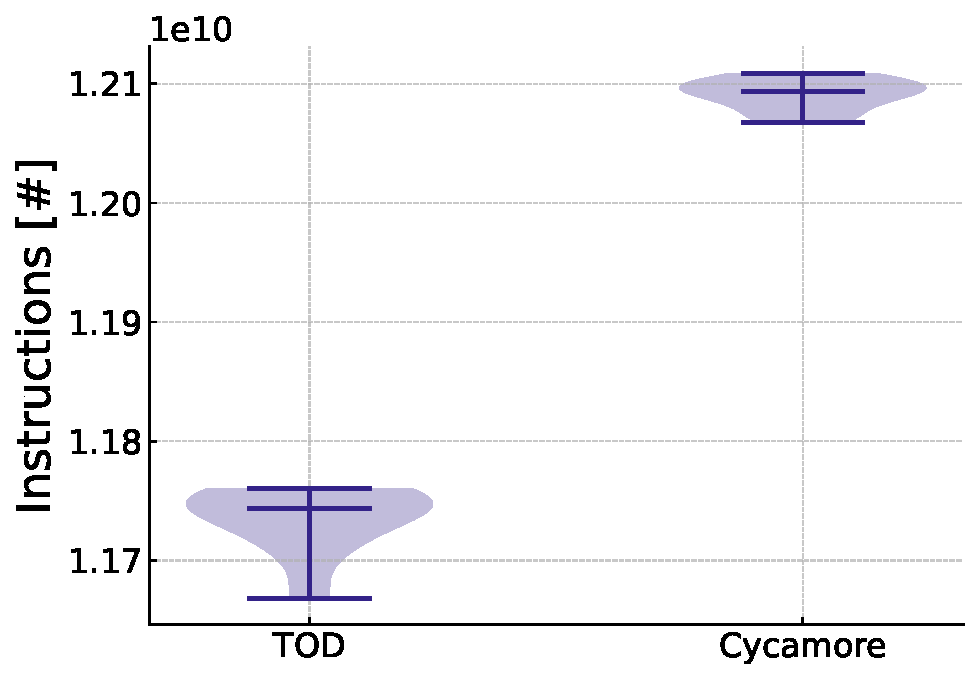
\includegraphics[width=1.01\textwidth]{images/ins_violin.pdf}
      \caption{Number of instructions for \gls{tod} and the \cycamore Reactor.}
      \label{fig:ins_tod_cyc}
    \end{figure}

    \column[t]{5cm}
    \begin{figure}[htbp!]
      \begin{center}
        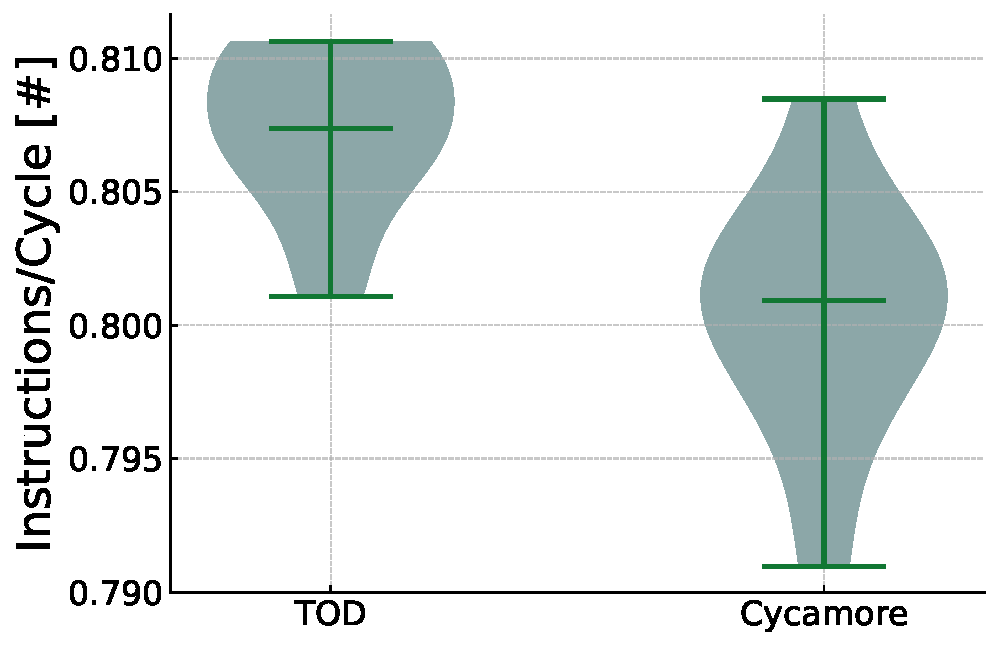
\includegraphics[width=1.065\textwidth]{images/ins_per_cyc.pdf}
      \end{center}
      \caption{Number of instructions per cycle for \gls{tod} and the \cycamore Reactor.}
      \label{fig:ins_per_cyc}
    \end{figure}
  \end{columns}
\end{frame}

\subsection{Future Work}
\begin{frame}
  \frametitle{Future work on DPR and \gls{tod}.}
  \begin{itemize}[<+->]
    \item Investigating the exchange method, and how the complexity can be streamlined.
    \item Applying trading on-demand and dynamic parameter logic to other standard fuel cycle archetypes where applicable.
    \item Incorporating other variations in the fuel usage (model hot or cold shut down, or off-cycle down powers).
    \item Generating synthetic power variation data based on the traditional LWR fleet performance and extrapolating that into the future.
    \item Attempting to create bounding cases that are an analogy to the performance of the advanced reactor designs we use in the work.
  \end{itemize}
\end{frame}

\section{Transition Scenarios}
  \subsection{LEU+ to HALEU}
  % \begin{frame}
  %   \frametitle{Our energy production is increasing.}
  %   \begin{figure}
  %       \centering
  %       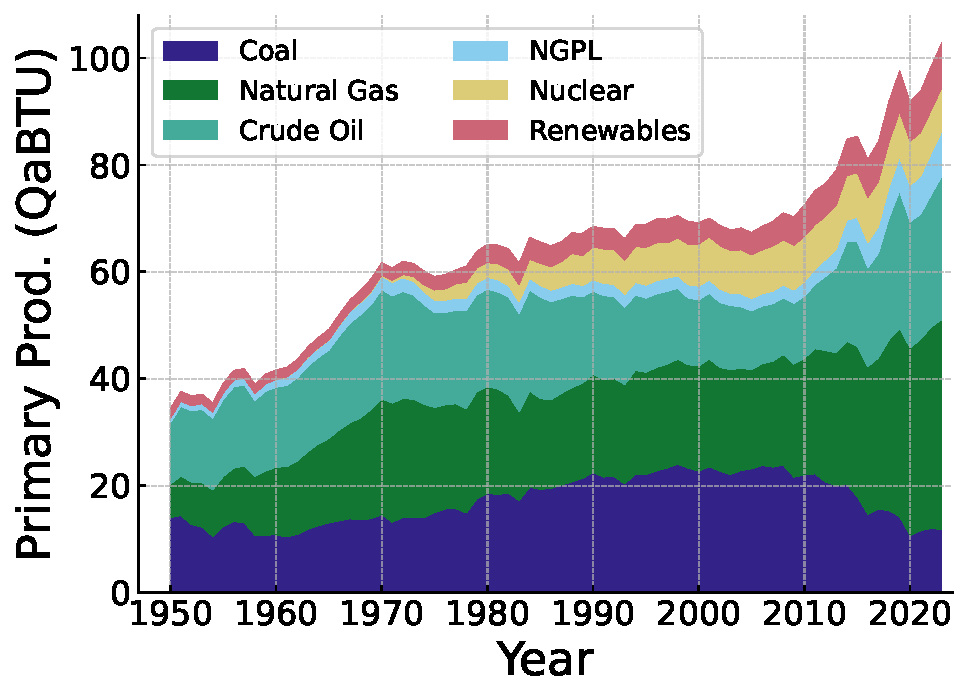
\includegraphics[width=0.65\textwidth]{images/prim_prod_b_source.pdf}
  %       \caption{1950-2023 Primary Energy Production by source. Reproduced from \cite{mer_april_2024}.}
  %   \end{figure}
  % \end{frame}

  \begin{frame}
    \frametitle{What if we can't get HALEU to fuel these advanced reactors?}
    \begin{figure}
        \centering
        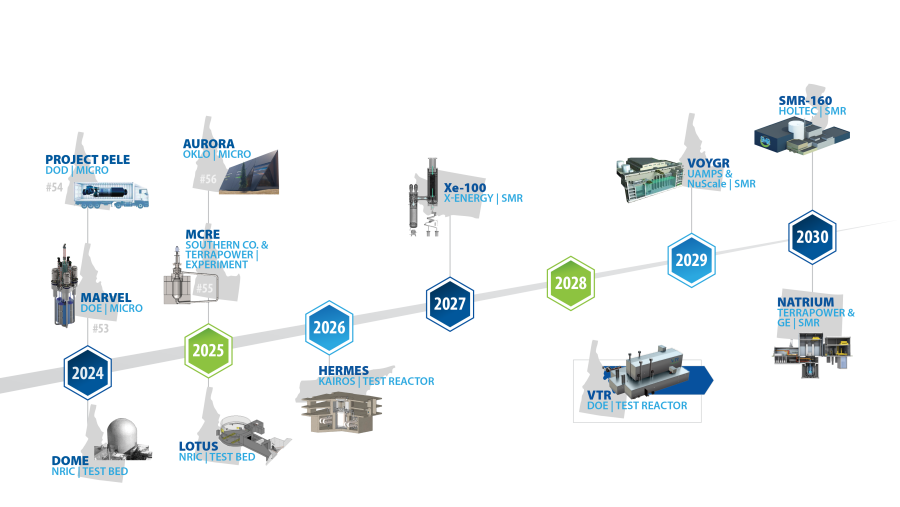
\includegraphics[width=0.86\textwidth]{images/reactor_timeline.png}
        \caption{Advanced reactor demonstration and deployment projects \cite{inl_reactor_timeline}.}
    \end{figure}
    Could we use \gls{leup} while HALEU supply chains develop?
  \end{frame}

  \begin{frame}
    \frametitle{We define LEU+ as 5-10\% $^{235}$U enrichment.}
    \begin{table}[H]
        \centering
        \caption{Enrichment levels and their ranges.}
        \label{tab:enrichment_levels}
        \begin{tabular}{c c}
          \hline
          \textbf{Enrichment Level} & \textbf{Range [\%  $^{235}$U]} \\
          \hline
          Natural & $<$ 0.711 \\
          LEU & 0.711-5 \\
          LEU+ & 5-10 \\
          HALEU & 10-20 \\
          HEU & $\geq$ 20  \\
          \hline
        \end{tabular}
    \end{table}
    These are a mash-up of economic and regulatory definitions.
  \end{frame}

  \begin{frame}
    \frametitle{We use Serpent to approximate reactors with LEU+ or HALEU.}
    \begin{columns}
      \column[t]{5cm}
      \begin{figure}
        \centering
        
\includegraphics[width=0.65\textwidth]{images/haleu_mmr_2blocks.inp_geom1.png}
        \caption{Top-down view of the \gls{leup} MMR core. Adapted from Bachmann \cite{bachmann_mmr_like_2023}.}
        \label{fig:td_mmr}
      \end{figure}

      \column[t]{5cm}
      \begin{figure}[htbp!]
        \begin{center}
          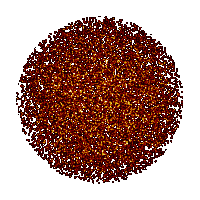
\includegraphics[width=0.65\textwidth]{images/htgr-mr-burn-200.inp_mesh1_bstep6.png}
        \end{center}
        \caption{Top-down view of the \gls{leup} Xe-100 core. Adapted from Richter \cite{richter_xe100_like}.}
        \label{fig:td_xe100}
      \end{figure}
    \end{columns}
  \end{frame}

  \subsection{Deployment Schemes}
  \begin{frame}
    \frametitle{We mimic real-world deployment by meeting energy demand.}
    \begin{figure}
      \centering
      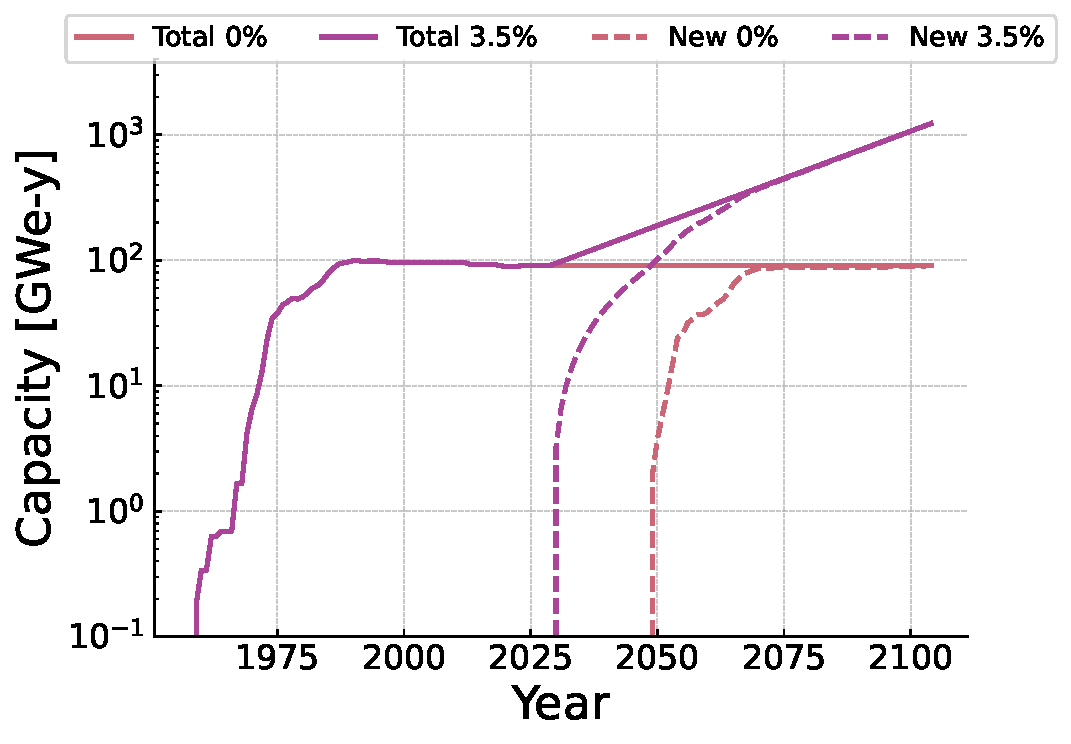
\includegraphics[width=0.65\textwidth]{images/new_capacity_ng_d2.pdf}
      \caption{Historical and projected US nuclear energy if we double the capacity of nuclear energy by 2050.}
    \end{figure}
  \end{frame}

  \begin{frame}
    \frametitle{Schemes have built-in assumptions about the scenario.}
    \begin{table}[H]
      \centering
      % \caption{Deployment schemes.}
      \label{tab:deployment_schemes}
      \newcommand{\ColWidth}{0.48\linewidth}
      \begin{tabular}{p{\ColWidth} p{\ColWidth}}
          \hline
          Scheme & Description \\
          \hline
          Greedy Deployment & Deploy reactors to fill demand, preferring to deploy larger capacity units first. \\
          \vspace{1.5mm}\\
          Random Deployment & Use the date and hour as seed to sample the
          reactors list randomly. \\
          \vspace{1.5mm}\\
          Initially Random, Greedy Deployment & Run the random scheme until
          a reactor bigger than the remaining capacity is proposed,
          then the greedy algorithm. \\
          \hline
      \end{tabular}
    \end{table}
  \end{frame}

  \begin{frame}
    \frametitle{Greedy reactor deployment scheme.}
    % \begin{algorithm}[H]
      \begin{algorithmic}[1]
        % \caption{Greedy Reactor Deployment Algorithm}
          \State Initialize demand
          \While{demand exists}
              \State Select the largest reactor that does not exceed demand
              \State Deploy reactors until the next reactor exceeds demand
              \State Update demand
          \EndWhile
      \end{algorithmic}\pause
    % \end{algorithm}
    So how does this idea of deferring HALEU demand by using LEU+ work in practice?
  \end{frame}

  % \begin{frame}
  %   \frametitle{Random reactor deployment scheme.}
  % %   \begin{algorithm}[H]
  % %     \caption{Random Reactor Deployment Algorithm}
  %     \begin{algorithmic}[1]
  %         \State Initialize demand
  %         \While{demand exists}
  %             \State Randomly deploy a reactor that does not exceed demand
  %             \State Update demand
  %         \EndWhile
  %     \end{algorithmic}
  % %     \end{algorithm}
  % \end{frame}

  % \begin{frame}
  %   \frametitle{Random + greedy reactor deployment scheme.}
  % %     \begin{algorithm}[H]
  % %       \caption{Random + Greedy Reactor Deployment Algorithm}
  %       \begin{algorithmic}[1]
  %           \State Initialize demand
  %           \While{demand exists}
  %               \State Randomly deploy a reactor
  %               \If{demand is exceeded}
  %                   \State Remove last reactor
  %                   \If{demand still exists}
  %                       \State Select the largest reactor that does not exceed demand
  %                       \State Deploy until the next reactor exceeds demand
  %                       \State Update demand
  %                   \EndIf
  %               \EndIf
  %           \EndWhile
  %       \end{algorithmic}
  % %       \end{algorithm}
  % \end{frame}

  \begin{frame}
    \frametitle{Staggering enrichment allows the supply chain to develop.}

    \begin{figure}
        \centering
        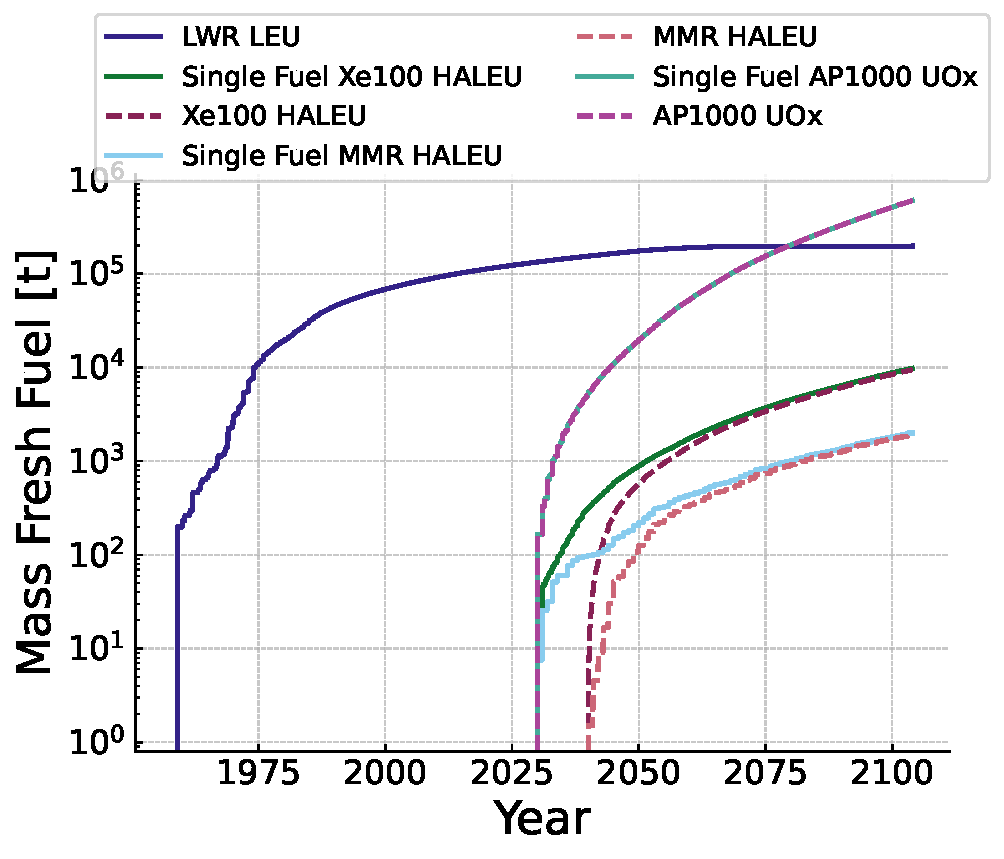
\includegraphics[width=0.6\textwidth]{images/fresh_fuel.pdf}
        \caption{The solid lines represent a scenario without LEU+, while the dashed lines represent a scenario with LEU+.}
    \end{figure}
  \end{frame}

  \begin{frame}
    \frametitle{The difference is on the order of hundreds of tonnes.}
    \begin{figure}
        \centering
        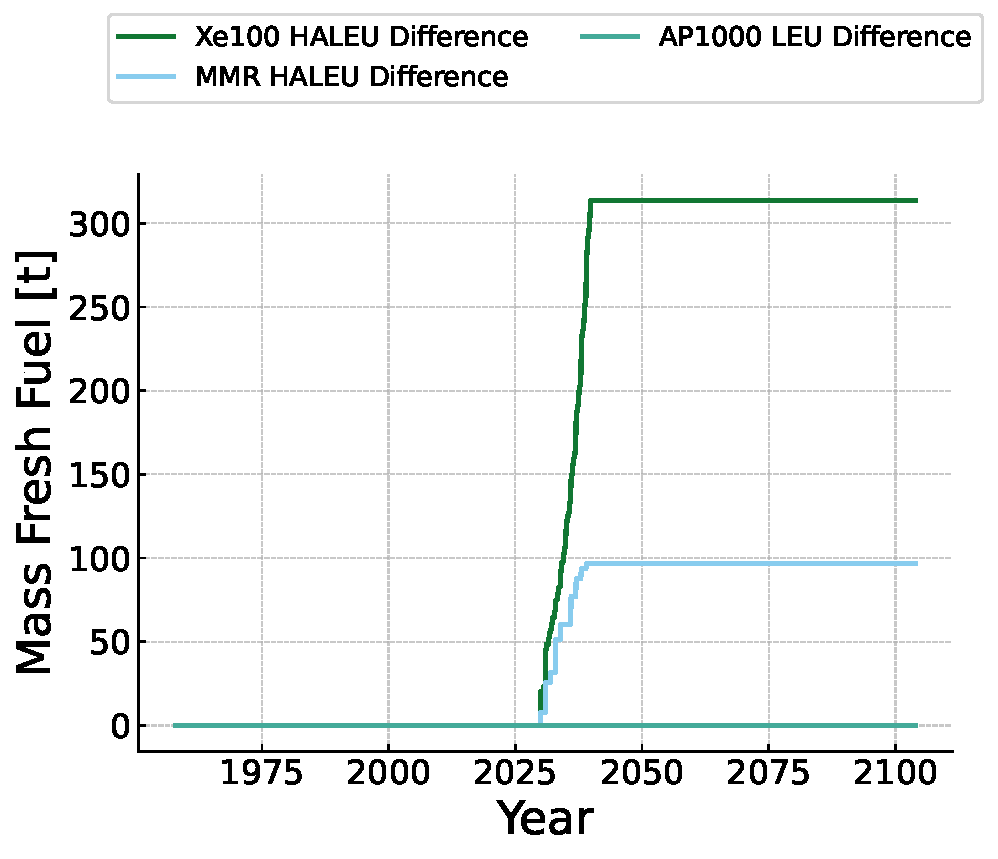
\includegraphics[width=0.65\textwidth]{images/fresh_fuel_difference.pdf}
    \end{figure}
  \end{frame}

  \begin{frame}
      \frametitle{Fuel cycle modeling is useful for enegy planning.}
      In our case, we transition from \gls{leup} to HALEU after 10 years of operation.
      \begin{itemize}
          \item For the Xe100 reactors, we need almost 315 less tonnes of HALEU.
          \item For the MMR reactors, we need almost 97 less tonnes of HALEU.
      \end{itemize}
      Next we need to characterize what the cost of this transition would be.
  \end{frame}

  \section{Big Questions}
  \begin{frame}
    \frametitle{\textit{Revisit:} \cyclus is being used to tackle big questions.}
    \begin{block}{Making transaction models more detailed.}
        Incorporate geospatial restrictions with OR-SAGE, the cost implications of my results, and multi objective optimization with OSIER \cite{Dotson_osier}.
    \end{block} \pause
    \begin{block}{Identifying realtime diversion or diversion paths.}
        Study tracer isotopes, such as $^{232}U$, suggested by Rhodes and Maldonado \cite{rhodes_u232}, and the effects of international collaboration on supply chain security.
    \end{block} \pause
    \begin{block}{Making facility models more accurate.}
      Continue \gls{ever}, and improve the exchange method's efficiency. Vary the power of coupled physics reactor models.
    \end{block}\pause
    \begin{block}{Finding advanced reactor impacts on the fuel cycle.}
      Consider how enrichment schemes, other reactor designs (including fusion), and the costs of fuel and waste management.
    \end{block}
  \end{frame}

  \begin{frame}
    \frametitle{More big questions.} % bad title
    \begin{block}{Reactor evOLutionary aLgorithm Optimizer (ROLLO)}
      Explore non-conventional geometries and fuel distributions to improve performance and safety.
    \end{block} \pause
    % \begin{block}{ATF fuel modeling.}
    %   I have a half-baked idea of modeling triso atf fuel? Or maybe ATF fuel cycles?
    % \end{block}
    \begin{block}{UNF isotope characterization and recycling.}

    \end{block} \pause
    \begin{block}{Nuclear-grade materials.}
      Characterizing the supply chain, and identifying opportunities for secondary material use.
    \end{block}
  \end{frame}

\begin{frame}
  \frametitle{Acknowledgements}
  This research was performed, in part, using funding received from the DOE
  Office of Nuclear Energy's Nuclear Energy University Program (Project 23-29656
  DE-NE0009390) 'Illuminating Emerging Supply Chain and Waste Management
  Challenges'.

  \vspace{0.5cm}

  This research was supported in part by an appointment to the Oak Ridge
  National Laboratory Research Student Internships Program, sponsored by the U.
  S. Department of Energy and administered by the Oak Ridge Institute for
  Science and Education.

  \vspace{0.5cm}

  Additionally, I would like to thank Luke Seifert for his help running the Serpent models.
\end{frame}




%%--------------------------------%%
%%--------------------------------%%
\begin{frame}[allowframebreaks]
  \frametitle{References}
  \bibliographystyle{plain}
  {\footnotesize \bibliography{bibliography.bib} }

\end{frame}
%%--------------------------------%%

\begin{frame}
  \frametitle{We have updated time, power, and deployment assumptions.}
    \textbf{Advanced Reactor Modeling:} Developed \gls{ever} reactor for flexible fuel loading and utilization.

    \vspace{8pt}
    \textbf{Dynamic Power Reactor (DPR):} Introduced DPR for more realistic energy demand modeling.

    \vspace{8pt}
    \textbf{On-Demand Fuel Trading (TOD):} Reduced computational complexity by optimizing reactor calculations.

    \vspace{8pt}
    \textbf{Transition Scenarios:} Examined supply chain flexibility and deployment schemes for advanced reactors, including LEU+ and HALEU.
\end{frame}

\end{document}
